\chapter{Modelo Estándar y Supersimetría}
% \addcontentsline{toc}{chapter}{Modelo Estándar y Supersimetría}
\chaptermark{Modelo Estándar y Supersimetría}

\section{Modelo estándar de la física de partículas}

El \textbf{Modelo Estándar} de la física de partículas (SM, por sus siglas en inglés) es la teoría que describe y clasifica a las partículas elementales de la naturaleza, junto con tres de las cuatro interacciones fundamentales conocidas hasta el momento. El mismo fue formulado en la década de los 70, a partir de varios trabajos científicos realizados durante la segunda mitad de ese siglo, entre los que se encuentra principalmente los realizados por Glasgow \cite{GLASHOW1961579}, Salam\cite{salam}, Weinberg\cite{PhysRevLett.19.1264}, Brout, Englert, Higgs\cite{PhysRevLett.13.321, PhysRevLett.13.508,PhysRevLett.13.585}. Para ese momento, el SM incorporaba a todas las partículas conocidas y postulaba la existencia de otras adicionales, lo que motivó al desarrollo de nuevos aceleradores y detectores para realizar dichas búsquedas. El descubrimiento de nuevas partículas e interacciones postuladas por el SM, junto con la medida de precisión de distintos parámetros del mismo, han convertido al SM en una teoría ampliamente aceptada por toda la comunidad científica, con una formulación matemática que sirve a su vez para nuevas futuras teorías.

\subsection{Partículas y clasificación del SM}

Las partículas en el SM se clasifican a primer orden entre \textbf{bosones} y \textbf{fermiones}. Los bosones de \textit{spin} 1 son los mediadores de las interacciones entre las distintas partículas del modelo. El primero de ellos es el fotón ($\gamma$), mediador de la interacción electromagnética, que afecta a las partículas que tienen carga eléctrica. No hay una fecha exacta del descubrimiento del mismo, pero se puede entender a la descripción del efecto fotoeléctrico por parte del Albert Einstein \cite{einstein}, como la primera formulación con objetos discretos de esta interacción. A su vez están los bosones asociados a la interacción débil, los bosones \Zzero y \Wpm, siendo estos últimos los que gobiernan los intercambios de `sabor' de las partículas. Propiamente fueron descubiertos (no sólo su interacción mediante corrientes cargadas y neutras) en 1983 en el Super Proton Synchrotron del CERN \cite{DiLella:2015yit}. Por otro lado se encuentran los gluones ($g$), mediadores de la interacción fuerte de aquellas partículas con carga de `color'. Existen tres cargas de color \textit{red}, \textit{green} y \textit{blue}, aunque las antipartículas pueden tener las anti cargas (\textit{antired}, \textit{antigreen} y \textit{antiblue}). Su primera observación experimental se realizó en 1978 en el detector PLUTO del colisionador electrón-positrón DORIS del DESY \cite{gluon}. Finalmente está el bosón de Higgs, partícula asociada al mecanismo Brout-Englert-Higgs que describe el rompimiento espontáneo de simetría electrodébil, asociado a la generación de masas de todas las partículas que componen al SM. El mismo fue descubierto en el 2012 por los experimentos ATLAS y CMS del CERN \cite{higgs_atlas, higgs_cms}. Cabe mencionar, que la bien conocida interacción gravitatoria, no es incluida en el SM debido a las contradicciones que aparecen al querer combinarla con la teoría de la Relatividad General. En teorías con gravedad cuántica, se hipotetiza la existencia de una partícula mediadora de esta fuerza denominada gravitón ($G$) y que se espera que sea no masiva y de spin 2.

Los fermiones están asociados a las partículas interactuantes o que forman la materia,
% (aunque no necesariamente tengan masa) % \solved{este comentario capaz se pueda omitir} Yep
esto se debe a que al obedecer la estadística de Fermi-Dirac, no es posible encontrarlos simultáneamente en un mismo estado cuántico y por ende tienden a formar estructuras. A su vez, estos se clasifican en \textbf{leptones} y \textbf{\textit{quarks}}. Los primeros son aquellos que no tienen carga de color y por ende no interactúan fuertemente. Existen seis leptones (junto con sus respectivas antipartículas): electrón ($e$), neutrino electrónico (\nue), muón ($\mu$), neutrino muónico (\numu), tau ($\tau$) y neutrino tauónico (\nutau), los cuales se agrupan en tres generaciones, que son pares de partículas que exhiben propiedades similares. Todos ellos pueden interactuar débilmente, y salvo por los neutrinos, también electromagnéticamente. Los quarks, en cambio, son los fermiones con carga de color, y por ende los que pueden interactuar fuertemente. Existen seis quarks (nuevamente junto con sus respectivas antipartículas) que se agrupan en tres generaciones: \textit{up} ($u$), \textit{down} ($d$), \textit{charm} ($c$), \textit{strange} ($s$), \textit{top} ($t$) y \textit{bottom} ($b$). Debido al efecto del confinamiento de color, los quarks nunca pueden ser observados en la naturaleza, sino que se los observa en estados ligados sin color, denominados hadrones. Cuando el hadrón se forma de un quark-antiquark se los llama mesones, y cuando es un conjunto de tres quarks se los llama bariones. Los bariones más conocidos son los protones ($p$) y neutrones ($n$), compuestos por los quarks de valencia $uud$ y $udd$ respectivamente, donde cada quark toma uno de los tres posibles colores. Toda la materia ordinaria observada (o estable) se compone de electrones, quarks up y down. Cabe destacar que es posible que en el presente texto se omita la diferenciación entre partícula y antipartícula, salvo cuando sea necesario hacerla explícita. Por ejemplo, es posible referirse al positrón como simplemente un electrón con carga positiva.
% \solved{Podría poner citas para los descubrimientos de los fermiones al igual que hice con los bosones...} No lo se... ya fue no... por completitud deberia estar pero son muchas particulas

Existe una clasificación adicional a partir de una propiedad intrínseca de las partículas denominada quiralidad. 
% La misma esta asociada al comportamiento de las funciones de onda en la teoría de Dirac frente a rotaciones espaciales. % \solved{omitir por confusion con helicidad}
Los fermiones pueden tener dos estados de quiralidad denominados izquierdo y derecho. Si bien en principio estos estados son posibles para todas los fermiones del SM, no se han observado experimentalmente neutrinos con quiralidad derecha\footnote{La quiralidad está íntimamente relacionada con la helicidad, y para partículas no masivas como el neutrino, son equivalentes}. Más aún, se observa que las interacciones cargadas electrodébiles son entre partículas izquierdas, 
% (o antipartículas derechas) % solved{no se por que pero sacarlo}
en lo que se denomina violación de paridad. Esto da a entender que en la naturaleza no hay una simetría entre las componentes izquierdas y derechas, y que teóricamente merecen un trato diferente.
En la Figura \ref{fig:sm_particles} se muestra un resumen de las partículas del SM junto con algunas de sus propiedades e interacciones.

\begin{figure}
  \centering
  \includegraphics[width=0.8\textwidth]{images/theory/sm_particles_4.pdf}
  \caption{Partículas del SM junto con el gravitón. Para cada una se indica su masa, carga eléctrica y spin. Por simplicidad las antípartículas fueron omitidas, y no se hace distinción entre partículas de quiralidad izquierda y derecha.}
  \label{fig:sm_particles}
\end{figure}


\subsection{Breve descripción matemática del SM}

El SM se formula como una teoría cuántica de campos, en general considerada efectiva, ya que por ejemplo, describe los fenómenos en una escala baja de energía en la que la gravedad es despreciable. A su vez, se compone de teorías de \textit{gauge} en las que a partir de imponer simetrías en el Lagrangiano, no solo están asociadas cantidades conservadas, como bien enuncia el Teorema de Emily Noether \cite{noether}, sino que también implica la existencia de interacciones mediadas por bosones de gauge. A continuación se realiza una breve descripción matemática del SM basada principalmente en la Referencia \cite{gkane}.

Hasta la actualidad, todos los experimentos demuestran que tres simetrías son necesarias y suficientes para describir todas las interacciones conocidas, sin incluir a la gravedad. Estas simetrías, otorgan a las distintas partículas respectivas cargas, que vienen a representar <<etiquetas>> que se les puede dar a las mismas, y que el conjunto de ellas describe en su totalidad a las propiedades de cada una.

El grupo de simetría del SM se define como:

\begin{equation}
	\mathcal{G}_{\text{SM}} = SU(3)_C \otimes SU(2)_L \otimes U(1)_Y
\end{equation}

La primer simetría a mencionar es la $SU(2)_L \otimes U(1)_Y$, relacionada con la interacción electrodébil. Los bosones de gauge requeridos por la invarianza de la teoría ante estas transformaciones son el $B_{\mu}$ y los $W_{\mu}^{i}$. El índice $\mu$ está presente debido a que los mismos deben transformarse bajo rotaciones espaciales de la misma forma que la derivada tradicional, garantizando así que las dichas partículas tengan spin 1. El índice $i$ representa cada uno de los tres bosones de spin 1, asociados a los tres generadores de las transformaciones $SU(2)$.

% \solved{reescrito}
% La primer simetría a mencionar es la $U(1)$, relacionada con la interacción electromagnética. El bosón de gauge requerido para mantener la invarianza se denomina $B_{\mu}$. El índice $\mu$ está presente debido a que $B_{\mu}$ debe transformarse bajo rotaciones espaciales de la misma forma que la derivada tradicional, garantizando así que la partícula tenga spin 1.
% A su vez, todas las partículas deben tener una segunda invarianza denominada $SU(2)$ electrodébil. Los bosones de gauge asociados se denominan $W_{\mu}^{i}$. El índice $i$ representa cada uno de los tres bosones de spin 1 asociados a los tres generadores de las transformaciones $SU(2)$.

Finalmente, la última simetría requerida es la $SU(3)_C$, con los bosones de gauge asociados $G_{\mu}^{a}$. El índice $a$ representa cada uno de los ocho bosones de spin 1, asociados a los ocho generadores de las transformaciones $SU(3)$. Estos bosones son los gluones, y la teoría que los describe es la cromodinámica cuántica (QCD).

Por su parte, los fermiones se describen mediante campos que definen estados dentro del espacio formado por las distintas simetrías. La simetría $SU(2)$ es análoga al spin, 
% \solved{reescrito}
% partículas con spin 0 son singletes, con spin $1/2$ forman dobletes y con spin 1 forman tripletes W^i con carga -1 0 y 1.
las partículas pueden formar singletes, dobletes o tripletes. % triplete forma el 
En el caso de $SU(2)$ electrodébil, los fermiones izquierdos forman dobletes, y los derechos forman singletes:

\begin{equation}
	f_L = 
	\begin{pmatrix}
	\nu_{e} \\
	e^{-} \\
	\end{pmatrix}_{L},
	\begin{pmatrix}
	u_\alpha \\
	d_\alpha \\
	\end{pmatrix}_{L}
	\quad\quad\quad
	f_R = e^{-}_{R},u_{R\alpha},d_{R\alpha}
\end{equation}

\noindent
donde por simplicidad, se omitieron los fermiones de la segunda y tercer familia.
Esta distinción entre izquierdos y derechos, es lo que hace que aparezca la violación de paridad electrodébil de forma natural en la teoría. El índice que aparece en los estados de los quarks, $\alpha$, es para describir cómo los mismos se transforman en el espacio $SU(3)$, de la misma forma que en $SU(2)$. En $SU(3)$ la representación fundamental son tripletes cuyas componentes representan los tres estados de color posible ($r$, $g$ y $b$). Los quarks forman tripletes,  mientras que los leptones son singletes sin color y por ello no requieren de este índice.
% \solved{Tal vez no sea correcto decir 'producto de la combinación de esos estados'} si, es correcto, no deberia estar eso, lo saque
% Gordon, pag 49.  
% If a particular color is “↑” in some direction, the combination analogous to ↑↓ (properly
% symmetrized) is colorless (just as a spin singlet can be constructed), so we speak of
% color (e.g. r) and anticolor (r̄) and color singlets (rr̄ + gḡ + bb̄). All leptons are color
% singlets so we have not written a color index for them. All quarks are color triplets.


Con esto en mente, el Lagrangiano se comienza a construir semejante al de una partícula libre, pero reemplazando la derivada ordinaria con la covariante, que con las simetrías consideradas, queda de la siguiente forma:


\begin{equation}
D_{\mu} = \partial_{\mu} - i g_{1} \frac{Y}{2}B_{\mu} - i g_{2} \frac{\tau^{i}}{2}W_{\mu}^{i} - i g_{3} \frac{\lambda^{a}}{2}G_{\mu}^{a}
\label{eq:cov_deriv}
\end{equation}

\noindent
donde $Y$, $\tau$ y $\lambda$ son los respectivos generadores de las transformaciones $U(1)$, $SU(2)$ y $SU(3)$, y $g_1$, $g_2$ y $g_3$ son constantes que representan la intensidad de cada acoplamiento y deben medirse experimentalmente. Se emplea una convención para escribir las ecuaciones de forma más compacta: los términos $D_{\mu}$ que actúen en los fermiones con una representación matricial diferente se anulan. Por ende, los $W_{\mu}^{i}$ (matrices $2\times2$ en $SU(2)$) que actúan sobre leptones derechos (singletes de $SU(2)$) se anulan, y los $G_{\mu}^{a}$ (matrices $3\times3$ en $SU(3)$) actuando sobre leptones (singletes de $SU(3)$) se anulan. Quedando así el término fermiónico del Lagrangiano:

\begin{equation}
\mathcal{L}_{\text{ferm}} = \sum_{\text{fermiones}} \bar{f}i\gamma^{\mu}D_{\mu}f
\end{equation}

Al desglosar los distintos términos de este Lagrangiano, es posible relacionar algunos de ellos tanto con observaciones experimentales, como con predicciones de la teoría. Por ejemplo, al mirar solo los términos $U(1)$ y $SU(2)$, se puede obtener el Lagrangiano asociado a la teoría electrodébil, donde se obtienen las denominadas corrientes neutras y cargadas, que posteriormente dieron con el descubrimiento de los bosones $W$ y $Z$. A su vez es posible obtener relaciones entre las constantes del modelo, entre las que se encuentra:

% / No hace falta... /
% \begin{equation}
% \begin{split}
% g_2 & = e/\sin{\theta_w} \\
% g_1 & = e/\cos{\theta_w}
% \end{split}
% \end{equation}
% %
% donde $\theta_w$ es un nuevo parámetro determinado experimentalmente, llamado ángulo de mezcla electrodébil. También la relación:

\begin{equation}
Q = T_3 + \frac{Y_W}{2} 
\end{equation}

\noindent
donde $Q$ es la carga eléctrica, $Y_W$ es el anterior mencionado generador de $U(1)$, que en este contexto se denomina hipercarga débil, y $T_3$ es la tercer componente del isospin débil. En caso de dobletes de $SU(2)$, los dos estados del mismo toman valores de $T_3$ igual $1/2$ o $-1/2$, y para singletes de $SU(2)$ toma un valor nulo.

De la misma forma se puede obtener el Lagrangiano asociado a QCD, mirando solo los términos $SU(3)$. Aún así no es posible sacar conclusiones de la misma forma que para la teoría electrodébil, debido al confinamiento de los quarks y gluones, que no permiten observarlos de forma aislada en la naturaleza. En la Sección \ref{sec:qcd_pp}, se describe de mejor forma algunos detalles de QCD, que resultan útiles a la hora de entender a las colisiones $pp$.

% Corregido: Por último cabe mencionar que en ningún momento se hizo distinción alguna entre las familias de leptones, por lo que es posible reemplazar en cualquier momento al electrón por el muón y lo mismo para su neutrino, y las ecuaciones siguen valiendo de la misma forma. 
Por último cabe mencionar que en ningún momento se hizo distinción alguna entre las familias de fermiones. Lo que permite, en las ecuaciones anteriores, reemplazar a los fermiones de la primer familia ($e$, $\nue$, $u$, $d$), por cualquiera de los de otras dos familias ($\mu$, $\numu$, $c$, $s$) o ($\tau$, $\nutau$, $t$, $b$), y las mismas seguirían teniendo validez.
Esto se denomina universalidad leptónica, y es una propiedad que ha sido de interés a lo largo de los años, en diferentes experimentos. Si la universalidad leptónica ha de cumplirse, los acoplamientos a los bosones de gauge debería ser iguales, y la única diferencia entre los leptones reside solo su masa. Una forma de medir este fenómeno es observando las fracciones de decaimiento a leptones de distintas partículas, como $\mu$, $\tau$ y principalmente hadrones con quarks bottom (hadrones $B$). Si bien en general las mediciones de estas fracciones están de acuerdo con las predicciones del SM, medidas recientes han observado desviaciones importantes\footnote{De aproximadamente 3-sigma, lo que en la jerga implica que aún no son significativas como para hablar de descubrimiento.} con respecto al mismo \cite{lepton_uni_1, lepton_uni_2}, lo que ha motivado el estudio de nuevas teorías que las expliquen (por ejemplo \textit{leptoquarks} \cite{leptoquark_1, Okumura:2744026}).


\subsection{Mecanismo de Higgs}

La formulación hasta ahora descripta no incluye en ningún momento las masas de ninguna de las partículas. Esto se debe a que al agregar términos de masa explícitos al Lagrangiano (como por ejemplo $m\psi\hat{\psi}$ o $m_B^2 B^{\mu}B_{\mu}$), el mismo pierde la invarianza electrodébil, ya que la misma sólo se garantiza poniéndole masa nula a todas las partículas. Si se incluyeran a las masas <<a mano>> la teoría termina teniendo cantidades físicas infinitas. 
% \solved{Entender, si es posible, por qué ocurre eso}. comentarios de ale
La forma más adecuada de incluir masas a la teoría
% sin que estas sean nulas % esto lo aclaro porque vengo de decir que la invarianza SU(2) la puedo salvar anulando las masas
es mediante el mecanismo de Higgs. Para ello se asume, que en el SM, el universo está inmerso en un campo de spin 0, denominado campo de Higgs. El mismo es un doblete en el espacio $SU(2)$, y tiene hipercarga no nula en $U(1)$, pero es un singlete en el espacio de color. 
% \solved{sacar y listo}
% Es un caso similar al del campo electromagnético, pero en el caso de Higgs no se consideran fuentes del campo en esta instancia. 
% Gordon, pag 13
% The field φ can be thought of as arising from a source in much the same way as the
% electromagnetic fields arise from charged particles; as for electromagnetism, we can
% consider the fields without concerning ourselves with the sources, although for scalars
% often the source is not so simple as a charged particle or body. In the Higgs physics
% case the Higgs field has no conventional source.
Los bosones de gauge y los fermiones pueden interactuar con este campo, y en su presencia dejan de tener masa nula. Si bien el Lagrangiano conserva la simetría $SU(2)$ y $U(1)$, el estado fundamental no, en lo que se denomina un rompimiento espontáneo de simetría.

La parte escalar del Lagrangiano de Higgs está dada por:

\begin{equation}
\mathcal{L} = (D^{\mu}\phi)^{\dagger}(D^{\mu}\phi) - V(\phi)
\end{equation}

\noindent
donde el $\phi$ es un campo escalar complejo en la representación de $SU(2)$:

\begin{equation}
	\phi = 
	\begin{pmatrix}
	\phi^{+} \\
	\phi^{0} \\
	\end{pmatrix} = \frac{1}{\sqrt{2}}
	\begin{pmatrix}
	\phi_{1} + i\phi_{2} \\
	\phi_{3} + i\phi_{4} \\
	\end{pmatrix}
\end{equation}

\noindent
con hipercarga $U(1)$, $Y=+1$. La derivada covariante en este término, es similar a la descripta en la Ecuación \ref{eq:cov_deriv}, pero sin el término de color, y con los mismos bosones de gauge de $SU(2)$ y $U(1)$. Esta simetría $U(1)_Y$ adicional, es necesaria para que la teoría genere un boson de gauge no masivo asociado al fotón.
$V(\phi)$ es el potencial de Higgs, que para garantizar la renormalización de la teoría e invarianza de $SU(2)$ y $U(1)$, requiere ser de la forma:

\begin{equation}
	V(\phi) = - \mu^{2}\phi^{\dagger}\phi + \lambda(\phi^{\dagger}\phi)^{2}
	\label{eq:higgs_pot}
\end{equation}

\noindent
donde $\lambda$ es un parámetro que debe ser mayor a $0$, para garantizar un mínimo del potencial, quedando el comportamiento determinado por el signo del otro parámetro, $\mu$. Para $\mu^2>0$, el campo genera un valor de expectación de vacío (VEV, $v:=\phi^{\dagger}\phi$) no nulo que rompe espontáneamente la simetría. El potencial $V(\phi)$ toma la forma de un sombrero mexicano (Figura \ref{fig:mexican_hat}), y tiene infinitos números de estados degenerados con energía mínima que satisfacen $v = \sqrt{-\mu^2/\lambda}$. De esos estados se elige arbitrariamente el estado:

\begin{equation}
	\left<\phi\right> = \frac{1}{\sqrt{2}}
	\begin{pmatrix}
	0 \\
	v \\
	\end{pmatrix}
\end{equation}

\begin{figure}
  \centering
  \includegraphics[width=0.6\textwidth]{images/theory/mexican_hat.png}
  \caption{Esquema del potencial de Higgs, cuya forma se asemeja a la de sombrero mexicano. Se puede apreciar que el mismo tiene infinitos estados de vacío degenerados, y uno es elegido durante la ruptura espontánea de simetría para el mecanismo de Higgs.}
  \label{fig:mexican_hat}
\end{figure}

Debido a la conservación de la carga, solo un campo escalar neutro puede adquirir VEV, por lo que $\phi^0$ se interpreta como la componente neutral del doblete, 
% \solved{el 'se interpreta' viene porque a piori no sabemos su carga, el 0 es notacion nomas}
y por ende $Q(\phi)=0$. El electromagnetismo no se modifica por el campo escalar VEV, y la ruptura de simetría se representa como:

\begin{equation}
SU(2)_L \otimes U(1)_Y \rightarrow U(1)_Q
\end{equation}

Para estudiar el espectro de partículas, se estudia al campo alrededor del mínimo utilizando una expansión en la dirección radial:

\begin{equation}
	\phi = \frac{1}{2}
	\begin{pmatrix}
	0 \\
	v + h \\
	\end{pmatrix}
\end{equation}

Al elegir una dirección particular, tenemos tres simetrías globales rotas, y por el teorema de Goldstone, aparecen tres bosones escalares no masivos. Estos bosones de Goldstone son absorbidos por los bosones $W$ y $Z$, adquiriendo así su respectiva masa, 
% \solved{esto es tecnicamente el mecanismo de higgs entonces?} si, los fermiones ganan masas por yukawa
mientras que la expansión en la dirección radial da la masa de la excitación $h$, que es la masa del boson de Higgs. De esta forma, queda la masa de los bosones de la teoría de la forma:

\begin{equation}
\begin{split}
	M_{\gamma} & = 0 \\
	M_{W} & = \frac{g_2 v}{2} \\
	M_{Z} & = \frac{v}{2}\sqrt{g_1^2 + g_2^2} \\
	M_{h} & = \sqrt{2\lambda}v \\
\end{split}
\end{equation}

% \solved{Creo que quedaría mejor m minúscula} Sip
% \solved{reescrito}
% Este mecanismo también permite otorgar masas a los fermiones, incluyendo en el Lagrangiano términos con acoplamiento del tipo Yukawa:
Los términos de acoplamiento del tipo Yukawa al campo de Higgs otorgan masas a los fermiones del SM:

\begin{equation}
	\mathcal{L}_{\text{Yuk}} = g_f(\bar{\psi}_L\phi \psi_R) + \text{h.c.}
\end{equation}

\noindent
siendo este, ahora sí, invariante electrodébil. 
% \solved{que otra invarianza? la completa del SM?} electrodebil
La constante $g_f$ describe el acoplamiento entre el doblete de Higgs y los fermiones. Al hacer una expansión del campo como se hizo anteriormente, aparecen en el Lagrangiano términos de masas fermiónicos que dan masa a los mismos de la forma:

\begin{equation}
m_f = \frac{g_f v}{\sqrt{2}}
\end{equation}

El mecanismo de Higgs da un cierre al SM, que queda completamente determinado por 19 parámetros\footnote{No se están contando los ángulos de mezcla y masas de los neutrinos} listados en la Tabla \ref{tab:sm_para}, los cuales deben ser medidos experimentalmente.


\begin{table} 
	
	\centering
	\begin{tabular}{ l | r }

	\hline	
	\hline

		Parámetro & Valor \\

		\hline
		\hline

    Masa del electrón $m_e$ & $0.511\,\mev$ MeV \\
    Masa del muón $m_{\mu}$ & $105.7\,\mev$ MeV \\
    Masa del tau $m_{\tau}$ & $1.78\,\gev$ \\
    Masa del up $m_u$ & $1.9$ MeV ($\mu_{\bar{\text{MS}}}=2\,\gev$) \\
    Masa del down $m_d$ & $4.4$ MeV ($\mu_{\bar{\text{MS}}}=2\,\gev$) \\
    Masa del strange $m_s$ & $87$ MeV ($\mu_{\bar{\text{MS}}}=2\,\gev$) \\
    Masa del charm $m_c$ & $1.32\,\gev$ ($\mu_{\bar{\text{MS}}} = m_c$) \\
    Masa del bottom $m_b$ & $4.24\,\gev$ ($\mu_{\bar{\text{MS}}} = m_b$) \\
    Masa del top $m_t$ & $173.5\,\gev$ (\textit{on-shell})\\
    Ángulo de mezcla de la matriz CKM ($\theta_{12}$) & $13.1\degree$ \\
    Ángulo de mezcla de la matriz CKM ($\theta_{23}$) & $2.4\degree$ \\
    Ángulo de mezcla de la matriz CKM ($\theta_{13}$) & $0.2\degree$ \\
    Fase de violación CP de la matriz CKM ($\delta$) & $0.995$ \\
    Constante de acoplamiento $U(1)$ ($g1$) & $0.357$ ($\mu_{\bar{\text{MS}}} = m_Z$) \\
    Constante de acoplamiento $SU(2)$ ($g2$) & $0.652$ ($\mu_{\bar{\text{MS}}} = m_Z$) \\
    Constante de acoplamiento $SU(3)$ ($g3$) & $1.221$ ($\mu_{\bar{\text{MS}}} = m_Z$) \\
    Parámetro de QCD ($\theta_{\text{QCD}}$) & ${\smallsim}0$ \\
    VEV del potencial de Higgs ($v$) & $246\,\gev$ \\
    Masa del Higgs ($m_h$) & $125.09\pm0.24\,\gev$ \\

    \hline
    \hline

	\end{tabular}
	\caption{Parámetros del SM y su valor experimental medido, donde en algunos se especifica la escala de la medida de dicho valor.}
	\label{tab:sm_para}
\end{table}


% \subsection{Renormalización}

% \soled{tesis de joaco.} NO VA
% Ale creo que sugiere no ponerlo....

% El SM es una teoría cuántica de campos renormalizable \cite{tesis_joaco}. Los efectos de órdenes superior
% introducen correcciones cuánticas, por ejemplo, en el cálculo de los acoplamientos
% en el SM, que deben tenerse en cuenta. Al mismo tiempo, las partículas en estos
% loops tienen momentos no acotados, por lo que surgen divergencias en los cálculos
% tanto para bajos momentos (llamadas infrarrojas o IR) como para altos momentos
% (ultra-violetas o UV), que deben eliminarse para que la teoría sea consistente con
% las mediciones experimentales. El proceso por el cual las divergencias desaparecen
% o se absorben al agregar una dependencia con la escala a los parámetros como
% los acoplamientos o masas de partículas, se conoce como renormalización. De esta
% forma el Lagrangiano físico, con los acoplamientos comparables con los experimentos,
% se puede escribir como un Lagrangiano desnudo (a distancias tendiendo a cero), menos un Lagrangiano que contenga los términos que eliminen las divergencias,
% a costo de introducir una dependencia con la escala $\mu$ del momento. Por tanto, la
% renormalización genera que los acoplamientos (y otros observables) no sean constantes y varíen con $\mu$. Tanto el screening en QED como la libertad asintótica y el
% confinamiento de QCD son consecuencias de este proceso de renormalización, que
% es a su vez una propiedad de las teorías de gauge.


\subsection{QCD y colisiones $pp$}\label{sec:qcd_pp}

Como se mencionó anteriormente, QCD \cite{qcd_collider, tesis_martin} es la teoría de campos de gauge renormalizable,
que describe la interacción fuerte entre quarks mediados por gluones. Los gluones son los objetos que generan las transiciones de un quark de color a otro. Las propiedades de los quarks en QCD, son análogas de alguna forma a las del fotón en QED, con la distinción de que estos sí llevan carga (de color). Esto genera que puedan autointeractuar, y además, cambiar la carga de color de los quarks (a diferencia de las partículas cargadas eléctricamente, que si bien pueden emitir o absorber un fotón, esto nunca cambia su carga). Esto se debe principalmente a la estructura no abeliana de su grupo de simetría.
Por otra parte, el grupo de renormalización afecta a la constante de acoplamiento fuerte ($\alpha_s$), que termina dependiendo de la distancia de las cargas o la energía de la interacción (\textit{running coupling constant}). 

En QED, la polarización del vacío es inducida por los
pares virtuales $e^{+}e^{-}$, que apantallan (\textit{screening}) la carga eléctrica y resulta en la disminución del
acoplamiento con la distancia. Por el contrario, los gluones no sólo producen pares $q\bar{q}$ (que causan un efecto análogo al de QED), sino que también crean pares de gluones adicionales,
que tienden a anti-apantallar (\textit{anti-screening}) la carga aparente de color. El efecto neto, es entonces, que el acoplamiento fuerte decrece con la energía y crece con la distancia. Esto da lugar al ya mencionado confinamiento de color, debido a que el potencial del campo de color aumenta linealmente con la distancia, y por lo tanto no se pueden observar quarks ni gluones libres en la naturaleza, solo observarlos en conjuntos sin color. Por otro lado, a pequeñas distancias o altas energías, se produce la libertad asintótica, donde la intensidad de
la interacción fuerte decrece, de tal forma que los quarks y gluones se comportan
esencialmente libres ($\alpha_s \ll 1$), posibilitando así un tratamiento perturbativo. 

Estas propiedades tienen un impacto directo a la hora de producir y observar quarks y gluones en un detector. Por ejemplo, en un colisionador de protones, los quarks y
gluones producidos altas energías, sufren un proceso conocido como <<hadronización>>,
a medida que pierden energía los mismos se van combinando con los quarks y antiquarks creados del vacío, formando hadrones. De esta forma no se detectan quarks o gluones de forma directa, sino que se observan como un chorro o cascada de partículas conocido como jets. Dichas cascadas en general se asemejan a un cono, con su vértice en el quark/gluon inicial, y agrupando todas las partículas producidas en dicha cascada. 




El LHC es principalmente un colisionador de protones, por lo que describir las interacciones que subyacen en la colisión misma, no solo es importante para entender los fenómenos que se producen, sino también para poder generar simulaciones de dichos procesos con una elevada precisión. Las colisiones $pp$, son ventajosas para obtener energías de colisión elevadas, pero con las desventaja de estar gobernadas principalmente por interacciones QCD, que son complejas en su propia naturaleza al realizar una descripción teórica. Para ello se utiliza el <<modelo de partones>>, introducido por Feynman \cite{feynman} y Bjorken \cite{bjorken} a fines de los años 60. 

El modelo de partones propone que a altas energías los hadrones están compuesto por partículas puntuales denominadas partones, que vienen a representar los quarks de valencia, y los quarks, antiquarks y gluones del mar, presentes en el protón. Cada uno de los partones lleva entonces una fracción de la energía y momento del protón, que a priori son desconocidas, lo que representa un problema a la hora de calcular secciones eficaces partónicas, $\sigma(qg\to qg)$.
Se suma además, en el caso de realizar una verificación experimental de la misma, el hecho de que los quarks y gluones del estado final no son observados de forma directa debido a la hadronización. En cambio, se calcula una sección eficaz hadrónica, $\sigma(pp\to jj)$, entre los protones incidentes y los jets del estado final. Para realizar este pasaje se emplea el teorema de factorización \cite{ELLIS1978281}, que permite una separación sistemática
entre las interacciones de corta distancia (de los partones), y las interacciones de larga distancia (responsables del confinamiento de color y la formación de hadrones). El teorema establece que la sección eficaz de producción de cualquier proceso de QCD del tipo $A+B\to X$, puede ser expresada como:

% \solved{Hasta el final, esta igual a la tesis de Tincho} Mala suerte

\begin{equation}
	\sigma_{AB\to X} = \sum_{ij} \int dx_{a_i} dx_{b_j} f_{A/a_i}(x_{a_i}, \mu_{F}^2) f_{B/b_j}(x_{b_j}, \mu_{F}^2) \sigma_{a_i b_j \to X}(\mu_{F}^2, \mu_{R}^2)
	\label{eq:xs_fact}
\end{equation}

\noindent
donde $x_i(x_j)$ es la fracción del momento del hadrón $A(B)$ que lleva el partón $a_i(b_j)$, y $\sigma_{a_i b_j \to X}$ es la sección eficaz de la interacción a nivel partónico, calculada a un dado orden en QCD perturbativo (pQCD) y una escala de renormalización $\mu_R$ \cite{tesis_martin}. La escala de renormalización es introducida
para absorber las divergencias ultravioletas, que aparecen en los cálculos perturbativos más
allá del primer orden.

Las funciones $f_{h/n}(x_{n}, \mu_{F}^2)$, llamadas funciones de distribución partónica (PDFs), representan la probabilidad de encontrar un partón de tipo $n$ en el hadrón $h$ con una fracción de
momento $x_n$, dada una escala de factorización $\mu_{F}$. Esta escala, es un parámetro arbitrario,
introducido para tratar singularidades que aparecen en el régimen no perturbativo. Estas
divergencias son absorbidas, en forma similar a la renormalización, dentro de las funciones
de distribución partónicas a la escala $\mu_F$. Si bien las PDFs no pueden ser determinadas
perturbativamente, se puede predecir su dependencia con $Q^2$, por medio de las ecuaciones
de evolución DGLAP (Dokshitzer-Gribov-Lipatov-Altarelli-Parisi) \cite{di_scattering,lipatov_parton,altarelli-parisi}. De esta forma, la
medida experimental de su forma funcional, a un dado $Q^2_0$ fijo, permite obtener predicciones
de las PDFs para un amplio espectro de $Q^2$. En la presente Tesis se consideran las predicciones teóricas a NLO utilizando las parametrizaciones CTEQ \cite{cteq}, MSTW \cite{mstw1, mstw2, mstw3} y NNPDF \cite{nnpdf}.

Luego de la interacción a alta energía, cada partón del estado final comienza a irradiar gluones,
perdiendo así energía. Estos gluones, nuevamente fragmentan en pares $q\bar{q}$ y gluones adicionales, y así sucesivamente, creando una lluvia de partones, de cada vez más bajo \pt. Esto continúa hasta
que la energía es suficientemente baja, y todos los partones se recombinan para formar
mesones y bariones, en lo que se conoce como hadronización. Las bajas transferencias de
energía involucradas en el proceso, son tales que este no puede ser tratado perturbativamente. La dinámica de esta evolución es absorbida en funciones de fragmentación, que
representan la probabilidad de un partón de fragmentar en un determinado hadrón del
estado final. La sección eficaz $\sigma_{AB\to X}$, en la Ecuación \ref{eq:xs_fact}, puede ser modificada entonces para
calcular el proceso $A + B \to C + X$:

\begin{equation}
	\sigma_{a_i b_j \to C+X} = \int dz_{C} D_{c_k}(z_C, \mu_{f}^2) \sigma_{a_i b_j \to c_k + X}(\mu_{F}^2, \mu_{R}^2)
\end{equation}

\noindent
donde $C$ es un hadrón, $D_{c_k}$ es la función de fragmentación, que define la probabilidad
de que un partón $c_k$ fragmente en un hadrón $C$, con una fracción $z_C$ de su momento a la
escala de fragmentación (o factorización del estado final) $\mu_{f}$. Esta escala es introducida
de manera similar a $\mu_{f}$ para el estado inicial, a fin de remover las singularidades por
radiación colineal en el estado final.

A lo largo de los años, en los distintos experimentos del LHC, se han realizado medidas de secciones eficaces de distintos procesos del SM. La Figura \ref{fig:sm_xs} muestra el buen acuerdo entre la sección eficaz medida en ATLAS de algunos procesos, y sus predicciones teóricas.

\begin{figure}
	\centering
  \includegraphics[width=0.8\textwidth]{images/theory/ATLAS_a_SMSummary_TotalXsect_3.pdf}
  \caption{Resumen de las distintas medidas de sección eficaz de algunos procesos del SM, comparadas con sus valores teóricos esperados \cite{sm_xs}.}
  \label{fig:sm_xs}
\end{figure}







\subsection{Limitaciones del Modelo Estándar}

En la sección anterior se describió brevemente la mayoría de las propiedades del SM junto con sus predicciones. A pesar de ser una de las teorías más exitosas de la 
% teoría cuántica de campos, 
física en general,
naturalmente el modelo tiene un rango de validez. A lo largo de los años la frontera experimental se ha ido expandiendo, observando nuevos (y no tan nuevos) fenómenos que la actual formulación del SM no puede explicar, principalmente en el rango de altas energías.

Una de las principales limitaciones del SM, es la imposibilidad de incluir a la gravedad de la misma forma que incluye a las demás interacciones. No solo incluir al gravitón a la teoría no es suficiente para poder explicar las observaciones, sino que la matemática empleada en el SM\footnote{Y de cualquier teoría cuántica de campos} es prácticamente incompatible con la formulación de la Relatividad General. Por otra parte, en el SM están presentes lo que se denominan problemas de jerarquía \cite{hierarchy}. 
% reescrito
% Un problema de jerarquía en el contexto de física de partículas, se refiere a cuando alguno de los parámetros empleados por la teoría difiere en varios ordenes de magnitud, de otros parámetros equivalentes de la misma. Esto lleva a pensar que la formulación de esa teoría no sea del todo definitiva, y que en cambio está compensando ciertos defectos incluyéndolos en ese parámetro tan diferente.  
Un problema de jerarquía en el contexto de física de partículas, se refiere a cuando alguno de los parámetros empleados en el Lagrangiano (masas o constantes de acoplamiento por ejemplo), difiere en varios ordenes de magnitud de su valor efectivo, que es el valor medido en un experimento. El valor efectivo esta relacionado con el valor fundamental a través de la renormalización, que aplica correcciones al mismo, y que en general ambos valores son cercanos.
Esto lleva a pensar que la formulación de esa teoría no sea del todo definitiva, y que en cambio, está compensando ciertos defectos, incluyéndolos en ese parámetro tan diferente. 
El caso más conocido tal vez, son los 17 órdenes de magnitud de diferencia entre la escala electrodébil ($M_W\sim 10^{2}\,\gev$) y el escala de Planck ($M_P\sim 10^{19}\,\gev$), en donde los efectos de la gravedad cuántica comienzan a ser comparables con las demás interacciones.

Por otro lado, observaciones cosmológicas sostienen que el SM solo describe casi el 5\% de la materia <<visible>>, y que existe un 25\% de materia que escapa la detección. Esta se denomina <<materia oscura>>, debido a que no es posible observarla mediante instrumentos que utilicen radiación electromagnética, pero sí a partir de sus efectos gravitatorios. El SM no provee una partícula candidata que logre cumplir todos los requisitos necesarios para ser materia oscura (eléctricamente nula y débilmente interactuante, entre otras cosas). Tampoco considera la asimetría bariónica, ya que en el universo abunda la materia con respecto a la antimateria, y el SM no es capaz de explicar dichas diferencias.

La observación de la oscilación de neutrinos, implica que si bien los neutrinos tienen una masa muy pequeña, la misma no es nula, en contraposición con lo que formula el SM. Si bien hay varios mecanismos para incluir las mismas dentro del SM, no hay evidencia suficiente para saber cuál es la forma correcta, 
sumado a que algunos modelos proponen la existencia de partículas adicionales aún no observadas \cite{MOHAPATRA_2005}.
% sumado a los nuevos desafíos teóricos que implica dicha inclusión (por ejemplo, existencia de nuevas partículas aun no observadas).

Por último, cabe destacar que varias magnitudes de la teoría, y medidas con una elevada precisión, han sido observadas desviándose de los valores predichos por el SM. Uno de especial interés en la actualidad, es la anomalía en la medida del momento dipolar magnético del muon (<<muon $g-2$>>) \cite{PhysRevLett.126.141801}. Estas diferencias no necesariamente significan un defecto en el SM, pero muchas veces puede ser una motivación para la formulación de nuevas teorías.

\section{Supersimetría}\label{sec:susy}

Retomando otro problema de jerarquía, el término de masa del Higgs recibe correcciones virtuales de cada partícula que se acople al campo de Higgs. 
% Considerando el potencial de la Ecuación \ref{eq:higgs_pot}, 
Si el campo de Higgs acopla a un fermión $f$ con un término en el Lagrangiano de la forma $-\lambda_f \bar{f} \phi f$, entonces el diagrama de Feynman que aparece en la Figura \ref{fig:loops} genera una corrección:

% solved{cito a esa ecuacion porque es la introduccion del martin} bueno no hacer
% \solved{Creo que quedaría mejor h minúscula} Se... convencion higgs siempre minuscula?

\begin{equation}
	\Delta m_h^2 = - \frac{|\lambda_f|}{8 \pi^2}\Lambda_{\text{UV}}^2 + ...
\end{equation}

\noindent
donde $\Lambda_{\text{UV}}$ es la escala de energía donde el SM deja de ser válido y nuevos fenómenos físicos pueden ser apreciables. Cualquier fermión del SM puede tomar el rol de $f$, pero la mayor corrección viene de parte del $top$ quark, con un $\lambda_f\sim1$, y un factor $3$ adicional por las cargas de color. Si $\Lambda_{\text{UV}}$ es del orden de $M_P$, las correcciones a la masa del Higgs son casi 30 órdenes de magnitud mayores a su valor medido. 
Inclusive, los demás bosones y fermiones del SM terminan siendo sensibles a esta escala, debido a que obtienen su masa a partir de $\left<H\right>$.
% Si bien los demás bosones y fermiones del SM no tienen este problema de forma directa, al obtener la masa a partir de $\left<H\right>$ terminan siendo sensibles a esta escala de la misma forma.

\begin{figure}
\centering

	\begin{subfigure}{0.45\textwidth}
	\begin{tikzpicture}
	\begin{feynman}
	\vertex (a) {\(H\)};
	\vertex [right=2cm of a] (b);
	\vertex [above right=of b] (e);
	\vertex [below right=of b] (f);
	\vertex [above right=of f] (c);
	\vertex [right=2cm of c] (d);
	\diagram* {
	(a)-- [scalar] (b),
	(b)-- [fermion, quarter left, edge label=\(f\)] (e),
	(e)-- [quarter left] (c),
	(c)-- [quarter left, fermion] (f),
	(f)-- [quarter left] (b),
	(c)-- [scalar] (d),
	};
	\end{feynman}
	\end{tikzpicture}
	\end{subfigure}
	\hfill
	\begin{subfigure}{0.45\textwidth}
	\begin{tikzpicture}
	\begin{feynman}
	\vertex (a) {\(H\)};
	\vertex [right=3cm of a] (b);
	\vertex [above left=of b] (d);
	\vertex [above right=of b] (f);
	\vertex [above right=of d] (e);
	\vertex [right=3cm of b] (c);
	\diagram* {
	(a)-- [scalar] (b),
	(b)-- [scalar, quarter left] (d),
	(d)-- [quarter left, scalar, edge label=\(S\)] (e),
	(e)-- [quarter left, scalar] (f),
	(f)-- [quarter left, scalar] (b),
	(b)-- [scalar] (c),
	};
	\end{feynman}
	\end{tikzpicture}
	\end{subfigure}

\caption{Correcciones cuánticas a un \textit{loop} al parámetro de masa del Higgs $m_{H}^{2}$ debido un fermión de Dirac \textit{f} (izquierda) y debido un campo escalar \textit{S} (derecha).}
\label{fig:loops}
\end{figure}

% \solved{mencionar alternativas para solucionar esto?} Nop
% 
% This is only directly a problem for corrections to the Higgs
% scalar boson squared mass, because quantum corrections to fermion and gauge boson masses do not
% have the direct quadratic sensitivity to Λ UV found in eq. (1.2). However, the quarks and leptons and
% the electroweak gauge bosons Z 0 , W ± of the Standard Model all obtain masses from hHi, so that the
% entire mass spectrum of the Standard Model is directly or indirectly sensitive to the cutoff Λ UV .
Una forma de solucionar esto es considerando la existencia de un escalar complejo $S$, con masa $m_S$, que acopla al Higgs mediante un término del Lagrangiano $-\lambda_S |\phi|^2|S|^2$, generando en el diagrama de la Figura \ref{fig:loops} una corrección del tipo:

\begin{equation}
	\Delta m_H^2 = - \frac{|\lambda_S|}{16 \pi^2}\left[\Lambda_{\text{UV}^2} - 2m_S^2 \ln{\Lambda_{\text{UV}}/m_S} + ... \right]
\end{equation}

Considerando la diferencia de signos entre el \textit{loop} fermiónico y bosónico, si cada fermión del SM estuviera acompañado por dos campos complejos con $\lambda_S = |\lambda_f|^2$, generaría una cancelación automática de los términos, eliminando de este modo las divergencias generadas. Esto motiva la inclusión de una nueva simetría a la teoría, entre fermiones y bosones, llamada \textbf{Supersimetría} (SUSY). Las secciones siguientes que describen la teoría supersimétrica fueron basadas en la Referencia \cite{martin}.

\subsection{Álgebra de SUSY}

Una transformación supersimétrica transforma un estado bosónico en uno fermiónico, y viceversa. El operador $Q$ que genera tal transformación, tiene que ser un espinor anticonmutativo:

\begin{equation}
	Q\ket{\text{Bosón}} = \ket{\text{Fermión}} \quad\quad\quad Q\ket{\text{Fermión}} = \ket{\text{Bosón}}
\end{equation}

Los espinores son objetos complejos, por lo que $Q^{\dagger}$ es también un generador de la simetría. Como $Q$ y $Q^{\dagger}$ son operadores fermiónicos (tienen spin $1/2$), supersimetría es una simetría espaciotemporal, y deben cumplir las siguientes reglas de (anti)conmutación:

\begin{equation}
	\begin{split}	
		\{Q,Q^{\dagger}\} & = P^{\mu}\\
		\{Q,Q\} & = \{Q^{\dagger},Q^{\dagger}\} = 0\\
		[P^{\mu},Q] & = [P^{\mu},Q^{\dagger}] = 0\\
	\end{split}	
\end{equation}
%
donde $P^{\mu}$ es el cuadrivector generador de las traslaciones espaciotemporales (los índices sobre los operadores $Q$ y $Q^{\dagger}$ fueron suprimidos intencionalmente).


Los estados de partícula son representaciones irreducibles del álgebra de SUSY, y se denominan <<supermultipletes>>. Cada uno contiene ambos estados bosónico y fermiónico, denominados <<supercompañeros>>. Como el operador $-P^2$ (cuyos autovalores son las masas) conmuta con los operadores $Q$ y $Q^{\dagger}$, y con los operadores de traslación y rotación, los supercompañeros dentro de un supermultiplete deben tener la misma masa. A su vez, como los operadores $Q$ y $Q^{\dagger}$ conmutan con los generadores de las transformaciones de gauge, los supercompañeros deben tener misma carga eléctrica, isospin débil y carga de color.

Cada supermultiplete debe contener igual número de grados de libertad fermiónica y bosónica, $n_F$ y $n_B$ respectivamente. Una forma posible de construir un supermultiplete con estas características es que tenga un solo fermión de Weyl con $n_F=2$ (dos estados de quiralidad),
% \solved{helicidad o quiralidad?} el martin dice quiralidad, lo paso a quiralidad por completitud ya fue
y dos campos escalares reales cada uno con $n_B=1$ (los cuales se combinan en un campo escalar complejo). Este tipo de supermultipletes de denominan escalares o quirales. Otra posibilidad es combinar un boson vectorial de spin 1 (boson de gauge no masivo con dos estados de quiralidad, $n_B=2$), con un fermión de Weyl no masivo de spin $1/2$ (con dos estados de quiralidad, $n_F=2$). Por como se transformar los bosones de gauge, sus supercompañero fermiónicos deben tener las mimas propiedades de las transformaciones de gauge para sus componentes izquierdas y derechas. Este tipo de supermultiplete se denominan vectoriales o de gauge. 
Si incluimos a la gravedad, entonces el gravitón de spin 2 ($n_B=2$) tiene un supercompañero con spin $3/2$, y si es no masivo con dos estados de quiralidad $n_F=2$. 
Hay otras posibilidades de partículas para generar supermultipletes, pero en general se terminan reduciendo a combinaciones de supermultipletes quirales y de gauge, excepto en teorías con supersimetrías adicionales. En nuestro caso inicial, la teoría se la denomina SUSY $N=1$, donde $N$ es el número de supersimetrías (o el número de conjuntos de operadores $Q$ y $Q^{\dagger}$). 

\subsection{El Modelo Estándar Supersimétrico Mínimo}

El \textbf{Modelo Estándar Supersimétrico Mínimo} (MSSM) es la extensión del SM que requiere incluir la mínima cantidad de partículas para completar los supermultipletes. Los supermultipletes solamente pueden ser escalares o vectoriales, y el spin de cada compañero debe diferir en $1/2$. Solo los supermultipletes escalares pueden contener fermiones cuyas partes izquierdas y derechas se transformen distinto frente a los grupos de gauge, y como los fermiones del SM tienen esta propiedad se los incluye en este tipo de supermultiplete. Cada componente izquierda y derecha de los fermiones son separadas en fermiones de Weyl con diferentes transformaciones de gauge, por lo que cada una tiene su compañero complejo escalar, un bosón de spin 0. Los nombres de estos bosones son iguales al de su fermión correspondiente, pero anteponiendo una <<s>> (por escalar en inglés), y lo mismo ocurre con su símbolo pero con una tilde. Tenemos entonces los los \textit{selectrons} (\selL, \selR), \textit{smuons} (\smuL, \smuR), \textit{squarks} (\squarkL, \squarkR), etc (también vale la terminología \textit{sleptons} ($\tilde{ell}$) o \textit{sfermions} ($\tilde{f}$) para el conjunto). Cabe mencionar que el índice en los sleptons representa la quiralidad del fermión correspondiente, y no su propia quiralidad (que no tienen por ser de spin 0). En el caso de los neutrinos, al ser siempre izquierdos, sus \textit{sneutrinos} no necesitan subíndice salvo para indicar su sabor: \snue, \snumu o \snutau. Las interacciones de los sfermions son las mismas que su correspondiente fermión, por lo que los $\tilde{f}_L$ acoplan con el bosón $W$ pero los $\tilde{f}_R$ no.

El bosón de Higgs debe encontrarse en un supermultiplete escalar debido a que tiene spin 0, pero a su vez el MSSM requiere de la existencia de dos dobletes escalares complejos de Higgs, en lo que se denomina el Modelo de Doble Doblete de Higgs (2HDM) Tipo II. A esos dobletes de $SU(2)_L$, con $Y=1/2$ e $Y=-1/2$, se los denomina $\Hu=(\Hup, \Huzero)$ y $\Hd=(\Hdzero, \Hdm)$ respectivamente. El bosón escalar de Higgs del SM es una combinación lineal de las componentes de isospin débil neutras de ambos dobletes ($\Huzero$ y $\Hdzero$). A los supercompañeros de los bosones se los nombra agregando el sufijo <<ino>> a su nombre, por lo que los supercompañeros de los dobletes de Higgs son los \textit{higgsinos}, $\Hinou=(\Hinoup, \Hinouzero)$ y $\Hinod=(\Hinodzero, \Hinodm)$.

Por otro lado, los bosones de gauge del SM deben estar contenidos en un supermultiplete vectorial, con sus respectivos supercompañeros denominados \textit{gauginos}. El gluon tiene un supercompañero de spin $1/2$, denominado \textit{gluino} ($\gluino$). Por su parte, la simetría $SU(2)_L\times U(1)_Y$ asociada a los bosones de gauge $\Wplus$, $W^0$, $\Wminus$ y $B^0$, tienen sus supercompañeros $\widetilde{W}^+$, $\widetilde{W}^0$, $\widetilde{W}^-$ y $\tilde{B}^0$, llamados \textit{winos} y \textit{bino}. Luego de la ruptura de simetría electrodébil, los estados de gauge $W^0$ y $B^0$ se mezclan en los estados de masa $\Zzero$ y $\gamma$, y de la misma forma lo hacen los $\widetilde{W}^0$ y $\widetilde{B}^0$, para dar lugar al \textit{zino} ($\widetilde{Z}^0$) y \textit{photino} ($\tilde{\gamma}$). Finalmente, y como se mencionó previamente, en caso de incluir a la gravedad, el gravitón ($G$) tiene su respectivo compañero, el \textit{gravitino} ($\gravino$).

En la Tabla \ref{tab:mssm_particles} se resume todas las partículas requeridas por el MSSM, donde vale remarcar que ninguno de los supercompañeros del SM mencionados anteriormente ha sido observado experimentalmente hasta la fecha. Otro comentario de interés, es que tanto el supermultiplete escalar \Hd (\Hdzero, \Hdm, \Hinodzero, \Hinodm), como el de los \sleptonL (\snu, \selL, $\nu_e$, $e_L$) tienen los mismos números cuánticos. Esto podría llevar a pensar que no es necesario incluir un nuevo doblete de Higgs y en cambio utilizar el de los sleptons$_L$. Si bien esto es posible, conlleva a diversos problemas fenomenológicos, como violaciones en el número de leptones y necesidad de neutrinos del SM muy masivos, lo que motiva a descartar esto.

% \solved{Faltaría el gravitino no?} done

\begin{table} 

	\centering

	\caption{Espectro de partículas del MSSM. Solo una de las tres familias de fermiones y sfermions es mostrada. 
	% Por convención, las componentes derechas de los mismos aparecen como conjugados/adjuntos. También al lado del nombre de los supermultipletes escalares aparece el símbolo para representar al supermultiplete como un todo. La barra arriba de los fermiones y sfermions derechos es parte del nombre, y no representa una conjugación. 
	}
	% \solved{Entender esto último y por qué la negrita y la barra en los números} ale comments
	\renewcommand{\arraystretch}{1.2}
	\begin{tabular}{ l c | c c c}

	\hline
	\hline

		\multicolumn{2}{l|}{Supermultipletes escalares} & Spin 0 & Spin $1/2$ & $SU(3)_C, SU(2)_L, U(1)_Y$ \\ 

		\hline
		\hline

		\multirow{3}{*}{squarks, quarks} & $Q$ & $(\tilde{u}_L\ \tilde{d}_L)$ & $(u_L\ d_L)$ & $(3, 2, \frac{1}{6})$ \\ [1ex]
		 & $u$ & $\tilde{u}_R$ & $u_R$ & $(3, 1, -\frac{2}{3})$ \\ [1ex]
		 & $d$ & $\tilde{d}_R$ & $d_R$ & $(3, 1, \frac{1}{3})$ \\ [1ex]

		\hline

		\multirow{2}{*}{sleptons, leptones} & $L$ & $(\tilde{\nu}_e\ \tilde{e}_L)$ & $(\nu_e\ e_L)$ & $(1, 2, -\frac{1}{2})$ \\ [1ex]
		 & $e$ & $\tilde{e}_R$ & $e_R$ & $(1, 1, 1)$ \\ [1ex]

		\hline

		\multirow{2}{*}{Higgs, higgsinos} & \Hu & $(\Hup\ \Huzero)$ & $(\Hinoup\ \Hinouzero)$ & $(1, 2, +\frac{1}{2})$ \\ [1ex]
		 & \Hd & $(\Hdzero\ \Hdm)$ & $(\Hinodzero\ \Hinodm)$ & $(1, 2, -\frac{1}{2})$ \\ [1ex]

		% \multicolumn{5}{c}{} \\

		\hline
		\hline

	\end{tabular}

	\vspace{0.5cm}

	\begin{tabular}{ l c | c c c}

		\hline
		\hline

		\multicolumn{2}{l|}{Supermultipletes vectoriales} & Spin $1/2$ & Spin 1 & $SU(3)_C, SU(2)_L, U(1)_Y$ \\

		\hline
		\hline

		\multicolumn{2}{l|}{gluino, gluon} & $\gluino$ & $g$ & $(8, 1, 0)$ \\ [1ex]
		\multicolumn{2}{l|}{winos, bosones $W$} & $\widetilde{W}^{\pm}\ \widetilde{W}^{0}$ & $W^{\pm}\ W^0$ & $(1, 3, 0)$ \\ [1ex]
		\multicolumn{2}{l|}{bino, bosón $B$} & $\widetilde{B}^0$ & $B^0$ & $(1, 1, 0)$ \\ [1ex]

		\hline
		\hline

	\end{tabular}
	\renewcommand{\arraystretch}{1}

	\label{tab:mssm_particles}

\end{table}


\subsection{Ruptura de SUSY}

Como se mencionó anteriormente, la formulación presentada hasta ahora del MSSM propone la existencia de nuevas partículas, cuyas masas son iguales a las masas de las partículas del SM. Por ejemplo, el \selL debería tener una masa de \magn{511}{keV}, el photino y gluino masas nulas, y lo mismo aplica para todas las demás partículas del SM, las cuales no superan los \magn{200}{GeV}. Este rango de energía ha sido ampliamente estudiado por distintos experimentos a lo largo de los años, y de existir partículas con esas masas, debería haber sido una tarea fácil detectarlas. Como no ha ocurrido, se asume que dichas partículas o tienen una masa muy baja y son poco interactuante, o tienen una masa muy grande, en un rango de energía aún no explotado. Se dice entonces que SUSY es una simetría débilmente rota, ya que se necesita esa ruptura para que aparezca la asimetría en masas, pero lo mínimo y necesario para preservar las características que solucionaban el problema de jerarquía. El Lagrangiano efectivo del MSSM toma la forma:

\begin{equation}
	\mathcal{L}_{\text{MSSM}} = \mathcal{L}_{\text{SUSY}} + \mathcal{L}_{\text{soft}} 
	\label{eq:l_susy}
\end{equation}

\noindent
donde $\mathcal{L}_{\text{SUSY}}$ contiene todas las interacciones de gauge y Yukawa, y preserva la invarianza frente a supersimetría, y $\mathcal{L}_{\text{soft}}$ viola supersimetría, pero contiene solo términos de masa y parámetros de acoplamiento con dimensiones positivas de masa. La diferencia de masas que hay entre las partículas del SM y sus supercompañeros, dependerá de la escala de masa más grande asociada al término \text{soft} ($m_{\text{soft}}$). Esta escala no puede ser indiscriminadamente grande ya que se perdería la solución al problema de jerarquía, y  las correcciones a la masa del Higgs serían extremadamente grandes. Se puede estimar 
% solved{Using Λ UV ∼ M P and λ ∼ 1 in eq Delta h} una estimacion aproximada con esta escala
que $m_{\text{soft}}$, y por ende las masas de los supercompañeros más livianos, deben estar en la escala del TeV. Esto es una de las motivaciones más importantes en las búsquedas experimentales, principalmente en los experimentos del LHC-CERN.


% / Interesante para poner, pero entender... /
% One might also wonder whether there is any good reason why all of the superpartners of the
% Standard Model particles should be heavy enough to have avoided discovery so far. There is. All of the
% particles in the MSSM that have been found so far, except the 125 GeV Higgs boson, have something
% in common; they would necessarily be massless in the absence of electroweak symmetry breaking. In
% particular, the masses of the W ± , Z 0 bosons and all quarks and leptons are equal to dimensionless
% coupling constants times the Higgs VEV ∼ 174 GeV, while the photon and gluon are required to be
% massless by electromagnetic and QCD gauge invariance. Conversely, all of the undiscovered particles
% in the MSSM have exactly the opposite property; each of them can have a Lagrangian mass term in the
% absence of electroweak symmetry breaking. For the squarks, sleptons, and Higgs scalars this follows
% from a general property of complex scalar fields that a mass term m 2 |φ| 2 is always allowed by all gauge
% symmetries. For the higgsinos and gauginos, it follows from the fact that they are fermions in a real
% representation of the gauge group. So, from the point of view of the MSSM, the discovery of the top
% quark in 1995 marked a quite natural milestone; the already-discovered particles are precisely those
% that had to be light, based on the principle of electroweak gauge symmetry. There is a single exception:
% it has long been known that at least one neutral Higgs scalar boson had to be lighter than about 135
% GeV if the minimal version of supersymmetry is correct, for reasons to be discussed in section 8.1. The
% 125 GeV Higgs boson discovered in 2012 is presumably this particle, and the fact that it was not much
% heavier can be counted as a successful prediction of supersymmetry.

En una teoría supersimétrica renormalizable, la interacción y las masas de todas las partículas están determinadas solamente por las propiedades de sus transformaciones de gauge y por el superpotencial $W_{\text{MSSM}}$. 
Del MSSM hasta ahora tenemos el grupo de gauge, las partículas del mismo y las propiedades de las transformaciones de gauge, resta describir entonces el superpotencial que toma la forma:

\begin{equation}
	W_{\text{MSSM}} = \bar{u}\textbf{y}_\textbf{u}QH_u - \bar{d}\textbf{y}_\textbf{d}QH_d - \bar{e}\textbf{y}_\textbf{e}LH_d + \mu H_u H_d
	\label{eq:susy_potential}
\end{equation}

Los campos que aparecen son los mismos de la Tabla \ref{tab:mssm_particles}, y las matrices $3\times3$ $\textbf{y}_\textbf{u}$, $\textbf{y}_\textbf{d}$, $\textbf{y}_\textbf{e}$, son los parámetros adimensionales del acoplamientos de Yukawa. Los índices para las transformaciones de gauge y familia de sabores fueron omitidos por practicidad. El último término, con el parámetro $\mu$, es la versión supersimétrica de la masa del Higgs del SM.

Por su parte, el término que describe el rompimiento de supersimetría de la forma más general toma la forma:

\begin{equation}
	\begin{split}
		\mathcal{L} = & -\frac{1}{2}\left( M_3 \gluino\gluino + M_2 \widetilde{W}\widetilde{W} + M_1 \widetilde{B}\widetilde{B} + c.c. \right) \\
			& - \left( \tilde{\bar{u}}\textbf{a}_\textbf{u}\widetilde{Q}H_u -  \tilde{\bar{d}}\textbf{a}_\textbf{d}\widetilde{Q}H_d -  \tilde{\bar{e}}\textbf{a}_\textbf{e}\widetilde{L}H_d + c.c. \right) \\
			& - \left( \squark^{\dagger} \textbf{m}_{\textbf{Q}}^{\textbf{2}}\squark - \tilde{L}^{\dagger}\textbf{m}_{\textbf{L}}^{\textbf{2}}\tilde{L} - \tilde{\bar{u}}\textbf{m}_{\bar{\textbf{u}}}^{\textbf{2}}\tilde{\bar{u}}^{\dagger} - \tilde{\bar{d}}\textbf{m}_{\bar{\textbf{d}}}^{\textbf{2}}\tilde{\bar{d}}^{\dagger} - \tilde{\bar{e}}\textbf{m}_{\bar{\textbf{e}}}^{\textbf{2}}\tilde{\bar{e}}^{\dagger} \right) \\
			& - m_{H_u}^2 H_u^* H_u - m_{H_d}^2 H_d^* H_d - (b H_u H_d + c.c.) \\
	\end{split}
\end{equation}

\noindent
donde $M_1$, $M_2$ y $M_3$ son los términos de masa del bino, wino y gluino, $\textbf{a}_\textbf{u}$, $\textbf{a}_\textbf{d}$ y $\textbf{a}_\textbf{e}$ son matrices complejas de $3\times3$ con unidades de masa.
% , se corresponden con los acoplamientos de Yukawa del superpotencial. 
% Martin, pag 61. They are in one-to-one correspondence with the Yukawa couplings of the superpotential.
El resto de los términos contienen los términos de masa de los sfermions y sector de Higgs.



\subsection{Mecanismos para la ruptura de SUSY}

% \solved{en la mitad es igual a la tesis de joaco} mala suerte...

% Anteriormente se mencionó una forma general para enunciar la ruptura de SUSY, y existen diferentes mecanismos para llevarla a cabo.
En el MSSM la ruptura de supersimetría simplemente se introduce explícitamente. Toda ruptura de una simetría global genera un modo no masivo de Nambu-Goldstone con los mismos números cuánticos que el generador de la simetría rota.
Para el caso de la supersimetría global, el generador es la carga fermiónica $Q_{\alpha}$,
por lo que la partícula de <<Nambu-Goldstone>> será un fermión de Weyl no masivo
neutro, llamado <<goldstino>>.
El rompimiento espontáneo de SUSY requiere un extensión del MSSM, agregando un sector oculto de partículas sin acoplamientos directos con los supermultipletes quirales del sector visible del
MSSM. Estos dos sectores comparten interacciones, que median el rompimiento de
SUSY desde el sector oculto al observable, como se esquematiza en la Figura \ref{fig:hidden_sector}, dando lugar a los términos soft del Lagrangiano del MSSM.
Las interacciones mediadoras entre el sector oculto y el observable pueden ser
de distinta naturaleza, por lo que existen muchos modelos que intentan explicar de
esta forma el rompimiento de SUSY. Uno de ellos es mediante interacciones gravitacionales, con modelos que se enmarcan en lo que se conoce como \textit{Planck scale mediated supersymmetry breaking} (PMSB), debido a que la gravedad entra cerca de la escala de Planck. Si SUSY se rompe en el sector oculto por un valor de expectación de vacío $\langle F \rangle$\footnote{$F$-term proveniente de los campos auxiliares $F$ incluidos al construir el Lagrangiano supersimétrico}, entonces los términos soft en el sector visible serán:

% \solved{Decir algo de F, Fterm}

\begin{figure}
  \centering
  \includegraphics[width=0.8\textwidth]{images/theory/hidden_sec.pdf}
  \caption{Estructura esquemática de la ruptura de supersimetría.}
  \label{fig:hidden_sector}
\end{figure}

\begin{equation}
m_{\text{soft}} \sim \left< F \right>/M_P
\label{eq:pmsb}
\end{equation}

Para $m_{\text{soft}}$ del orden de ${\smallsim}100\,\gev$, la escala de rompimiento de SUSY en el sector oculto es $\sqrt{\langle F \rangle}\sim 10^{11}\,\gev$.
Cuando se tiene en cuenta la gravedad, SUSY deber ser una simetría local y la
teoría se conoce como supergravedad. En este caso, el gravitón de espín $2$ tiene un
supercompañero fermión de espín $3/2$, el gravitino, inicialmente no masivos. Una vez
que SUSY es espontáneamente rota, el gravitino absorbe al goldstino, adquiriendo
masa, que se convierte en sus componentes longitudinales (helicidad $\pm1/2$). La masa
del gravitino $m_{3/2}$, se puede estimar de la Ecuación \ref{eq:pmsb}, y se espera que sea comparable a la masa de las partículas del MSSM (entre \magn{100}{GeV} y \magn{1000}{GeV} aproximadamente).

Si se considera interacciones de gauge electrodébiles y QCD ordinarias, se tienen
los modelos \textit{Gauge Mediated Supersymmetry Breaking} (GMSB) \cite{gmsb1, gmsb2, gmsb3} (se considera aquí que estas interacciones siempre dominan sobre gravedad). Los términos
soft del MSSM provienen de diagramas a un loop que involucran partículas mensajeras, que son nuevos supermultipletes quirales que se acoplan al VEV $\langle F \rangle$ que
rompe SUSY, y tienen a su vez interacciones $SU(3)_C \times SU(2)_L \times U(1)_Y$ que generan
la conexión con el MSSM. Se tiene en este caso:

\begin{equation}
m_{\text{soft}} \sim \frac{\alpha_a}{4\pi}\frac{\langle F \rangle}{M_\text{mens}}
\label{eq:gmsb}
\end{equation}

\noindent
donde $\alpha_a$ es el factor de loop para diagramas de Feynman involucrando interacciones de gauge, y $M_\text{mens}$ es la escala característica de las masas de los campos mensajeros. En
caso que $M_\text{mens}$ y $\left< F \right>$ sean comparables, se pueden tener $m_{\text{soft}}$ en el correcto
orden de magnitud con sólo $\sqrt{\left< F \right>}\sim 10^4\,\gev$.

El marco más general se conoce como General Gauge Mediation (GGM), en el
cual se define al mecanismo de mediación por campos de gauge como el límite en
que las constantes de acoplamiento del MSSM $\alpha_a\to 0$, la teoría se desacopla en el
MSSM y un sector oculto separado que rompe SUSY. Como característica principal, la masa del
gravitino es $m_{3/2} \ll M_W$, típicamente del orden del eV, lo que implica que es la \textbf{Partícula Supersimétrica Más Liviana} (LSP, por sus siglas en inglés) 
de la teoría. Es interesante notar que debido a que la LSP es siempre el gravitino, la
partícula más liviana del MSSM es la NLSP (\textbf{Siguiente Partícula Supersimétrica Más Liviana}) de la teoría, y su naturaleza determina
entonces el estado final que se encuentra en un colisionador.

\subsection{Paridad R}

El superpotencial de la ecuación \ref{eq:susy_potential} es mínimamente suficiente para producir la fenomenología necesaria para el modelo. Sin embargo, existen otros términos que se pueden incluir que si bien cumplen los requisitos, no se los incluye debido a que violan el número bariónico ($B$) o el leptónico ($L$). Por ejemplo:

\begin{equation}
	\begin{split}
		W_{\Delta B = 1} & = \frac{1}{2}\lambda ''^{ijk}\bar{u}_i\bar{d}_j\bar{d}_k \\
		W_{\Delta L = 1} & = \frac{1}{2}\lambda^{ijk}L_iL+j\bar{e}_k + \lambda^{ijk}L_iQ_j\bar{d}_k + \mu '^{i}L_i H_u \\
	\end{split}
	\label{eq:lb_viol}
\end{equation}

Los supermultipletes $Q$ tienen $B=+1/3$, los $\bar{u}_i$ y $\bar{d}_i$ tienen $B=-1/3$ y el resto $B=0$, en cambio los $L_i$ tienen $L=+1$, los $\bar{e}_i$ tienen $L=-1$ y el resto $L=0$. Por lo que la primer igualdad de la Ecuación \ref{eq:lb_viol} viola el número bariónico en una unidad, y la segunda el número leptónico en una unidad. En caso de cumplirse esa relación el protón tendría la posibilidad de decaer, por ejemplo a un pion y un electrón, en una fracción muy pequeña de tiempo. Esto contradice las observaciones experimentales, donde se ponen cotas superiores al tiempo de vida media mayores a $10^{32}$ años. Motivada por esta y otras conservaciones, se podría postular directamente la conservación de $B$ y $L$ directamente en el MSSM, pero esto sería un retroceso con respecto al SM, donde esta conservación sale de forma 
% `natural'
<<accidental>>
. Para resolver esto se introduce una nueva simetría, que elimina la posibilidad de una violación de $B$ y $L$:

\begin{equation}
	P_R = (-1)^{3(B-L)+2s}
\end{equation}

\noindent
donde $s$ es el spín de la partícula. Las partículas del SM más los bosones de Higgs tienen $P_R = +1$, mientras que el resto de las partículas del MSSM tienen $P_R = -1$. Si $P_R$ se conserva, no puede haber mezcla entre las partículas con $P_R$ opuestos, y cada vértice de interacción de la teoría debe tener un número par de partículas con $P_R=-1$. Esto a su vez implica que la LSP debe ser completamente estable. En caso de ser la LSP neutra, debe interactuar débilmente con la materia ordinaria y por ende es un candidato interesante para materia oscura. Por otro lado, cada partícula supersimétrica que no sea la LSP, debe decaer a un estado con número impar de partículas supersimétricas, que eventualmente termina en la LSP. También a partir de esta simetría se puede concluir que en experimentos de colisión las partículas supersimétricas son producidas de a número par, generalmente de a dos.



\subsection{Espectro de masa del MSSM}

Como ocurre en el SM, los estados de gauge que se muestran en la tabla \ref{tab:mssm_particles} no son necesariamente los estados de masa que se pueden observar experimentalmente, sino combinaciones de los mismos. En el MSSM no es una tarea trivial obtener los distintos autovalores de masa, ya que ahora hay dos dobletes complejos de Higgs, y varios conjuntos de partículas con los mismos números cuánticos que pueden dar una mezcla. La Figura \ref{fig:susy_part} resume los estados de gauge y masa del MSSM, los cuales se listan a continuación.

\begin{figure}
  \centering
  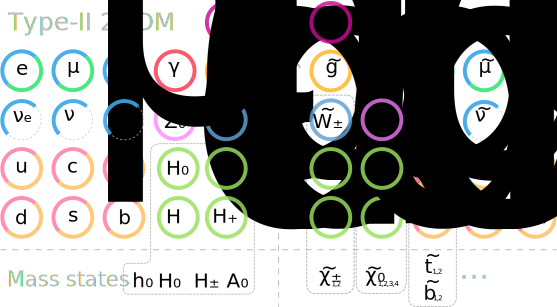
\includegraphics[width=0.9\textwidth]{images/theory/sm_susy_v2.pdf}
  \caption{Estados de gauge y masa del MSSM. A la izquierda de muestran las partículas del 2HDM SM ($P_R = +1$), y a la derecha sus respectivos supercompañeros ($P_R = -1$). Las partículas del SM que pueden tener dos estados de quiralidad se representan con dos colores, y ambos estados tienen sus respectivos supercompañeros con su mismo color. Las correspondientes antipartículas no son mostradas explícitamente. Debajo se muestran algunos de los posibles estados de masa. El $G$ y \gravino fueron incluidos por ser de particular interés para esta tesis.}
  % \tosolve{el graviton y gravitino son del mssm tecnicamente?}
  \label{fig:susy_part}
\end{figure}

\subsubsection{Neutralinos y charginos}

Los higgsinos y los gauginos electrodébiles se mezclan debido a la ruptura de la simetría electrodébil. Los higgsinos neutrales (\Hinouzero y \Hinodzero) y los gauginos neutrales ($\widetilde{B}$, $\widetilde{W}^0$) se combinan para formar cuatro estados de masa llamados neutralinos (\ninoone, \ninotwo, \ninothree, \ninofour). Los higgsinos cargados (\Hinoup y \Hinodm) y los winos ($\widetilde{W}^+$, $\widetilde{W}^-$) se combinan para formar dos estados de masa con carga, llamados charginos (\chinoonepm, \chinotwopm). Por convención se utiliza el subíndice para ordenarlos de forma ascendente a partir de su masa. En general se supone al neutralino más liviano, \ninoone, como la LSP ya que es la única partícula del MSSM que es buen candidato a materia oscura\footnote{Esto no ocurre en modelos con gravitinos más livianos, o con violación de la paridad R}. A partir de los estados de gauge, los valores de las masas se obtienen entonces diagonalizando las matrices que entran en el término de masa del Lagrangiano. En el caso de los neutralinos, la matriz $4\times4$ no es fácil resolver analíticamente. Una de las posibles aproximaciones, propone que la ruptura de simetría electrodébil se puede considerar como una pequeña perturbación en la matriz de masa de los neutralinos. Asumiendo entonces que: 

\begin{equation}
	m_Z \ll |\mu \pm M_1|, |\mu \pm M_2|
\end{equation}

\noindent
se obtienen neutralinos prácticamente <<bino-like>> ($\ninoone \approx \widetilde{B}$), <<wino-like>> ($\ninotwo \approx \widetilde{W}^0$) y <<higgsino-like>> ($\ninothree, \ninofour \approx (\Hinouzero \pm \Hinodzero)/\sqrt{2}$), con autovalores:

\begin{equation}
	\begin{split}
		m_{\ninoone} = & M_1 - \frac{m_Z^2 s_W^2 (M_1 + \mu \sin{2\beta})}{\mu^2 - M_1^2} + ... \\
		m_{\ninotwo} = & M_2 - \frac{m_W^2 (M_2 + \mu \sin{2\beta})}{\mu^2 - M_2^2} + ... \\
		m_{\ninothree} = & |\mu| + \frac{m_Z^2 (\text{sign}(\mu) - \sin{2\beta})(\mu + M_1 c_W^2 + M_2 s_W^2)}{2 (\mu + M_1) (\mu + M_2)} + ... \\
		m_{\ninofour} = & |\mu| + \frac{m_Z^2 (\text{sign}(\mu) + \sin{2\beta})(\mu - M_1 c_W^2 - M_2 s_W^2)}{2 (\mu - M_1) (\mu - M_2)} + ... \\
	\end{split}
	\label{eq:nc_mass}
\end{equation}

\noindent
donde $M_1$ y $M_2$ se asumen reales y positivos, y $\mu$ real que puede ser tanto positivo como negativo. 
Un parámetro que aparece en las masas es el ángulo $\beta$, que se define a partir de los valores de expectación de vacío de $H_u^0$ y $H_d^0$:
	
\begin{equation}
	\tan(\beta) \equiv \frac{v_u}{v_d} = \frac{\left< H_u^0 \right>}{\left< H_d^0 \right>}
\end{equation}

El subíndice de cada neutralino debe ser acomodado de tal forma de que queden ordenados por su masa. La misma aproximación se puede realizar con los charginos\footnote{Aunque esta matriz sí tiene solución analítica: \\ $m_{\chinoonepm, \chinotwopm}^2 = \frac{1}{2} \left[ |M_2|^2 + |\mu|^2 + 2 m_W^2 \mp \sqrt{(|M_2|^2 + |\mu|^2 + 2 m_W^2)^2 - 4 |\mu M_2 - m_W^2 \sin{2\beta}|^2} \right]$} que terminan siendo <<wino-like>> y <<higgsino-like>> con masas:

\begin{equation}
	\begin{split}
		m_{\chinoonepm} = & M_2 - \frac{m_W^2 (M_2 + \mu \sin{2\beta})}{\mu^2 - M_2^2} + ... \\
		m_{\chinotwopm} = & |\mu| + \frac{I m_W^2 (\mu + M_2 \sin{2\beta})}{\mu^2 - M_2^2} + ... \\
	\end{split}
\end{equation}

\subsubsection{Gluinos, squarks y sleptons}

El gluino no puede mezclarse con ninguna otra partícula del MSSM debido a
que es un fermión de color de ocho componentes. La masa la obtiene del término de ruptura de SUSY incluido en $\mathcal{L}_{\text{soft}}$, cuyo parámetro de masa es $M_3$.

Para el caso de los squarks y sleptons, como en principio todo escalar con la misma carga eléctrica, paridad R y color puede mezclarse entre sí, los estados de masa se obtienen diagonalizando las tres matrices de masa cuadrada de $6\times6$ para los squarks de tipo `up' ($\tilde{u}_L$, $\tilde{c}_L$, $\tilde{t}_L$, $\tilde{u}_R$, $\tilde{c}_R$, $\tilde{t}_R$), de tipo `down' ($\tilde{d}_L$, $\tilde{s}_L$, $\tilde{b}_L$, $\tilde{d}_R$, $\tilde{s}_R$, $\tilde{b}_R$), sleptons cargados ($\tilde{e}_L$, $\tilde{\mu}_L$, $\tilde{\tau}_L$, $\tilde{e}_R$, $\tilde{\mu}_R$, $\tilde{\tau}_R$), y la matriz de $3\times3$ para sleptons neutros ($\tilde{\nu}_e$, $\tilde{\nu}_{\mu}$, $\tilde{\nu}_{\tau}$). Las partículas de la tercer familia tienen masas bastante diferentes a las de la primera y segunda, e inclusive tienen mezclas significativas principalmente mediante los pares ($\tilde{t}_L, \tilde{t}_R$), ($\tilde{b}_L, \tilde{b}_R$) y ($\tilde{\tau}_L, \tilde{\tau}_R$), cuya combinación genera los $\tilde{t}_{1,2}$, $\tilde{b}_{1,2}$ y $\tilde{\tau}_{1,2}$ respectivamente. En cambio, los de la primera y segunda familia forman siete pares casi degenerados sin mezcla ($\tilde{e}_R, \tilde{\mu}_R$), ($\tilde{\nu}_e, \tilde{\nu}_\mu$), ($\tilde{e}_L, \tilde{\mu}_L$), ($\tilde{u}_R, \tilde{c}_R$), ($\tilde{d}_R, \tilde{s}_R$), ($\tilde{u}_L, \tilde{c}_L$) y ($\tilde{d}_L, \tilde{s}_L$).





\subsubsection{Escalares de Higgs}

Los campos de Higgs escalares en le MSSM se componen de dos dobletes de $SU(2)$ complejos, con ocho grados de libertad. Cuando ocurre la ruptura de simetría electrodébil tres de ellos son los bosones de Nambu-Goldstone, que se convierten en los modos longitudinales de los bosones $Z^0$ y $W^{\pm}$. Los cincos restantes consisten en dos escalares neutrales CP-par $h^0$ y $H^0$, un escalar neutral CP-impar $A^0$, y dos escalares cargados $H^+$ y $H^-$. Por convención $h^0$ es el más liviano, y se lo designa como bosón de Higgs del SM. Las masas de los mismos se pueden escribir como:

% \solved{la masa de h0 y H0 son iguales?} nop, hay un mas menos ahi

\begin{equation}
	\begin{split}
		m_{A^0}^2 = &\ 2b/\sin(2\beta) \\
		m_{h^0 , H^0}^2 = &\ \frac{1}{2}\left( m_{A^0}^2 + m_Z^2 \mp \sqrt{(m_{A^0}^2-m_Z^2)^2 + 4m_Z^2 m_{A^0}^2 \sin^2(2\beta)} \right) \\
		m_{H^{\pm}}^2 = &\ m_{A^0}^2 + m_W^2 \\
	\end{split}
\end{equation}


\subsection{Decaimientos de las partículas supersimétricas}

A continuación se describen los posibles decaimientos de las partículas supersimétricas. En general se asume que se conserva la paridad R y se considera al \ninoone como la LSP, aunque también se describe el caso donde el \gravino es la LSP.

\subsubsection{Decaimientos de los neutralinos y charginos}

Los posibles decaimientos de los neutralinos y charginos pueden ser:

% \begin{equation}
% 	\begin{split}
% 		\tilde{N}_i \to &\ Z\tilde{N}_j,\ W\tilde{C}_j,\ h^0\tilde{N}_j,\ l\tilde{l},\ \nu\tilde{\nu},\ [A^0\tilde{N}_j,\ H^0\tilde{N}_j,\ H^{\pm}\tilde{C}_j^{\mp},\ q\squark] \\
% 		\tilde{C}_i \to &\ W\tilde{N}_j,\ Z\tilde{C}_j,\ h^0\tilde{C}_1,\ l\tilde{\nu},\ \nu\tilde{l},\ [A^0\tilde{C}_1,\ H^0\tilde{C}_1,\ H^{\pm}\tilde{N}_j,\ q\squark'] \\
% 	\end{split}
% \end{equation}

\begin{equation}
	\begin{split}
		\ggino^0_i \to &\ \Zboson\ggino^0_j,\quad \Wmp\ggino^\pm_j,\quad h^0\ggino^0_j,\quad \ell\slepton,\quad \nu\snu,\quad [\Azero\ggino^0_j,\quad \Hzero\ggino^0_j,\quad \Hpm\ggino^\mp_j,\quad q\squark] \\
		\ggino^\pm_i \to &\ \Wpm\ggino^0_j,\quad \Zboson\ggino^\pm_j,\quad h^0\chinoonepm,\quad \ell\snu,\quad \nu\slepton,\quad [\Azero\chinoonepm,\quad \Hzero\chinoonepm,\quad \Hpm\ggino^0_j,\quad q\squark'] \\
	\end{split}
\end{equation}

Los estados en corchetes son los que están mayormente suprimidos cinemáticamente. Puede ocurrir también que todos estos decaimientos a dos cuerpos estén cinemáticamente prohibidos para un cierto gaugino, principalmente \chinoonepm y \ninotwo. En ese caso pueden ocurrir decaimientos a tres cuerpos de forma \textit{off-shell} a partir de bosones de gauge, escalares de Higgs, sleptons y squarks:

\begin{equation}
	\ggino^0_i \to ff\ggino^0_j,\quad \ggino^0_i \to ff'\ggino^\pm_j,\quad \ggino^\pm_i \to ff'\ggino^0_j,\quad \chinotwopm \to ff\chinoonepm
\end{equation}

\noindent
donde $f$ es una notación genérica para los leptones y quarks, y $f'$ es el otro miembro del multiplete de $SU(2)_L$. La Figura \ref{fig:susy_three_body_decays} muestra los diagramas de decaimientos a los estados finales más comunes de los neutralinos y charginos.



\begin{figure}[H]
  \centering
  \includegraphics[width=0.8\textwidth]{images/theory/nc_decays.png}
  \caption{Decaimientos a tres cuerpos más comunes de los neutralinos y charginos.}
  \label{fig:susy_three_body_decays}
\end{figure}

\subsubsection{Decaimientos de los gluinos, squarks y sleptons}

El gluino solo puede decaer a través de un squark, ya sea \textit{on-shell} o virtual. Si el decaimiento a
dos cuerpos está abierto, este va a dominar debido a que el acoplamiento gluino-quark-squark tiene intensidad de QCD.
En el caso de que todos los squarks sean más pesados que el gluino, este va a decaer solo vía
squarks virtuales.



\begin{equation}
	\begin{split}
		\gluino\to &\ q\squark \\
		\gluino\to &\ qq\ggino^0_i,\ qq\ggino^\pm_i \\
	\end{split}
	\label{eq:gluino_dec}
\end{equation}


Por otro lado, los decaimientos posibles de los sfermions son:

\begin{equation}
	\begin{split}
		\slepton \to &\ \ell\ggino^0_i,\quad \slepton \to \nu\ggino^\pm_i,\quad \snu\to \nu\ggino^0_i,\quad \snu\to \ell\ggino^\pm_i \\
		\squark\to &\ q\gluino,\quad q\ggino^0_i,\quad q'\ggino^\pm_i
	\end{split}
\end{equation}

\subsubsection{Decaimientos a gravitinos}

Como se mencionó anteriormente, en modelos como GGM la LSP es el gravitino. En general, el decaimiento $\widetilde{X} \to X\gravino$ no compite frente a los otros posibles decaimientos de la sparticles, excepto cuando esta es la NLSP, ya que esta necesariamente debe decaer al gravitino más su supercompañero. De particular interés es cuando la NLSP es el $\ninoone$, en ese caso los posibles decaimientos son a $\gamma\gravino$, $Z\gravino$, $h^0\gravino$, $A^0\gravino$ y $H^0\gravino$. De estos decaimientos, los últimos dos son muy poco probables cinemáticamente.
% , y el primero es el único cinemáticamente garantizado \tosolve{Habría que ver bien qué significa esto} % no lo entiendo, creo que se refiere a que el decaimiento a foton siempre esta, pero entra en contradiccion con el modelo de EWK
Los decaimientos a $Z^0$ y $h^0$, están sujetos a una fuerte supresión cinemática proporcional a $ (1-m_{Z}^{2}/m_{\ninoone}^{2})^4$ y $(1-m_{h^{0}}^{2}/m_{\ninoone}^{2})^4$, pero aún juegan un papel importante en la fenomenología si $ \langle F \rangle $ no es demasiado grande (${\lesssim}10^9\,\tev$), \ninoone tiene un contenido considerable de zino o higgsino, y $m_{\ninoone}$ es significativamente mayor que $m_{Z}$ o $m_{h^{0}}$. 
% \solved{Esto lo puse también en el capitulo de EWK, capaz mejor queda aca} Oka
En general, la probabilidad de decaimiento del \ninoone depende de los parámetros de mezcla de los neutralinos, del ángulo de Weinberg y también de su masa, a partir de los parámetros que las definen en las Ecuaciones \ref{eq:nc_mass}.

\subsection{Producción de partículas supersimétricas en colisionadores de hadrones}

Asumiendo la conservación de la paridad R, en colisionadores de hadrones, las partículas supersimétricas pueden producirse de a pares a partir de colisiones de partones con interacciones fuertes:

\begin{equation}
	\begin{split}
		gg\to &\ \gluino\gluino,\ \squark_i\squark_j^* \\ 
		gq\to &\ \gluino\squark_i \\ 
		q\bar{q}\to &\ \gluino\gluino,\ \squark_i\squark_j^* \\ 
		qq\to &\ \squark_i\squark_j \\ 
	\end{split}
\end{equation}

\noindent
o interacciones electrodébiles:

\begin{equation}
	\begin{split}
		q\bar{q}\to &\ \ggino_i^+\ggino_j^-,\ggino_j^0\ggino_j^0 \quad\quad u\bar{d}\to\ggino_i^+\ggino_j^0 \quad\quad d\bar{u}\to\ggino_i^-\ggino_j^0 \\
		q\bar{q}\to &\ \slepton_i^{+}\slepton_j^{-},\snu_l\snu_l^* \quad\quad u\bar{d}\to\sleptonL^{+}\snu_l \quad\quad d\bar{u}\to\sleptonL^{-}\snu_l^* \\
	\end{split}
\end{equation}

En la Figura \ref{fig:sp_production} se puede observar los principales diagramas de Feynman de las distintas producciones. En la Figura \ref{fig:susy_xs} se muestras las secciones eficaces de producción de los distintos procesos, donde se manifiesta que la producción electrodébil tiene una sección eficaz notablemente menor a la fuerte.

\begin{figure}
  \centering
  \includegraphics[width=0.8\textwidth]{images/theory/sp_production.png}
  \caption{Algunos ejemplos de diagramas de Feynman de producción de partículas supersimétricas en colisionadores de hadrones. Las tres de arriba representan la producción electrodébil de gauginos, mientras que el resto la producción fuerte de gluinos y squarks.}
  \label{fig:sp_production}
\end{figure}

\begin{figure}
  \centering
  \includegraphics[width=0.8\textwidth]{images/theory/SUSY_xsecs_13TeV_overview.pdf}
  \caption{Sección eficaz de producción de partículas supersimétricas en colisiones $pp$ \cite{susy_xs}.}
  \label{fig:susy_xs}
\end{figure}


Las búsquedas de SUSY realizadas por la colaboración ATLAS hasta la fecha han impuesto límites en la sección eficaz de producción y masas de las partículas supersimétricas, considerando diferentes tipos de producción y canales de decaimiento. La Figura \ref{fig:susy_xs_limits} resume algunos de estos resultados obtenidos hasta Junio de 2021.


\begin{figure}
	\centering
  \includegraphics[width=0.95\textwidth]{images/theory/susy_xs_limits.pdf}
  \caption{Estado actual de los límites obtenidos para las masas de las partículas supersimétricas, considerando diferentes tipos de producción y canales de decaimiento \cite{susy_xs_limits}.}
  \label{fig:susy_xs_limits}
\end{figure}